\documentclass{article}
\usepackage[utf8]{inputenc}
\usepackage{url}
\usepackage{amsmath,amsthm,enumitem}
\usepackage{graphicx}
\usepackage{lscape}
\usepackage{geometry}
\usepackage{color}
\usepackage{float}
\usepackage{listings}
\usepackage{amssymb}
\usepackage{verbatim}
\usepackage{algpseudocode} 
\usepackage{algorithm}
\usepackage{algorithmicx}  
\usepackage{hyperref}
\usepackage{courier}
\usepackage{listings} 
\usepackage{subcaption}
\usepackage{algorithm,algpseudocode}
\renewcommand{\baselinestretch}{1.5}
\DeclareMathOperator*{\argmax}{arg\,max}
\DeclareMathOperator*{\argmin}{arg\,min}
\geometry{left=2.5cm,right=2.5cm,top=2.5cm,bottom=2.5cm} 
% \renewcommand{\baselinestretch}{2}
\setcounter{MaxMatrixCols}{20}
\algnewcommand{\Inputs}[1]{%
  \State \textbf{Inputs:}
  \Statex \hspace*{\algorithmicindent}\parbox[t]{.8\linewidth}{\raggedright #1}
}
\algnewcommand{\Initialize}[1]{%
  \State \textbf{Initialize:}
  \Statex \hspace*{\algorithmicindent}\parbox[t]{.8\linewidth}{\raggedright #1}
}

\theoremstyle{definition}
\newtheorem{definition}{Definition}

\theoremstyle{plain}
\newtheorem{theorem}{Theorem}
\newtheorem{lemma}{Lemma}
\newtheorem{remark}{Remark}
\newcounter{example}[section]
\newenvironment{example}[1][]{\refstepcounter{example}\par\medskip
   \noindent \textbf{Example~\theexample. #1} \rmfamily}{\medskip}

\title{Note on Matching}
\author{Haocheng Dai}
\date{}
\DeclareUnicodeCharacter{2212}{-}
\begin{document}
\maketitle


\section{Large Deformation}
\subsection{Landmark Matching\cite{joshi,miller,johnson}}
\subsubsection{Problem formulation}
Assuming that there is a set of landmarks $\{(x_n,y_n)\}$, where $x_n$ and $y_n$ are  our approach is to construct diffeomorphisms $\phi:\Omega\rightarrow\Omega$, such that
\begin{align}
    \hat{v}(x,t)&=\argmin_vE(v)+D(\phi(\cdot,1))\\ \nonumber
    &=\argmin_v \int^1_0\sum_{n=1}^N\|Lv(x_n,t)\|^2_{L^2}dt+\sum^N_{n=1}[y_n-\phi(x_n,1)]^T\Sigma^{-1}_N[y_n-\phi(x_n,1)],
\end{align}
where
\begin{align*}
    \phi(x,0)&=x\\
    \phi(x,1)&=x+\int^1_0\Dot{\phi}(x,t)dt\\
    \Dot{\phi}(x,t)&=\frac{d\phi(x,t)}{dt}=v(\phi(x,t),t)=v_t\circ\phi_t
\end{align*}

The final time diffeomorphism $\phi(\cdot,1)$ is controlled via the velocity field $v(\cdot,t),t\in[0,1]$. Diffeomorphic landmark transformations are constructed by forcing the velocity fields to minimize quadratic energetic on $\Omega\times[0,1]$, as shown below
\begin{align*}
    E(v)&=\int_0^1\int_\Omega\|Lv(x,t)\|^2_{L^2}dxdt\\
    &=\int_0^1\int_\Omega\sum^{d}_{q=1}|(-\nabla^2+c)v_q(x,t)|^2dxdt
\end{align*} 
since $L$ is in form of $L=I\cdot(-\nabla^2+c)$, where $I$ is the identity matrix, $d$ is the dimension of $v$ and $c$ is a constant.

The squared error distance for landmark matching is given by
\begin{equation*}
    D(\phi(\cdot,1))=\sum^N_{n=1}[y_n-\phi(x_n,1)]^T\Sigma^{-1}_n[y_n-\phi(x_n,1)],
\end{equation*}
where $\Sigma_N$ is the error covariance.

\subsubsection{Inexact Landmark Matching}
$L$ is a constant coefficient matrix differential operator with $d\times d$ matrix Green's function $G(x,y)$ which is continuous in both $x$ and $y$. Let $K(x,y)=GG^\dagger(x,y)=(2/\sqrt{2\pi c})e^{-\sqrt{c}\|x-y\|}$, where $K$ is a $d\times d$ matrix function. $K$ is the Green's kernel\cite{ref2}. 
Given $N$ pairs of landmarks $\{\phi(x_i,1),x_i\}$, we are going to generate the vector field in form of
\begin{equation*}
    \hat{v}(x,t)=\sum^N_iK(\phi(x_i,t),x)\cdot w_i
\end{equation*}
under the $N$ constraints that
\begin{align*}
    \hat{v}(x_1,t)&=\sum^N_iK(\phi(x_i,t),x_1)\cdot w_i\\
    &\vdots\\
    \hat{v}(x_N,t)&=\sum^N_iK(\phi(x_i,t),x_N)\cdot w_i
\end{align*}

Incorporating all the constraints above in a matrix form, we can have the equation below
\begin{equation*}
    \underbrace{
    \begin{pmatrix}
    K(\phi(x_1,t),\phi(x_1,t))&\cdots&K(\phi(x_1,t),\phi(x_N,t))\\
    \vdots&\ddots&\vdots\\
    K(\phi(x_N,t),\phi(x_1,t))&\cdots&K(\phi(x_N,t),\phi(x_N,t))
    \end{pmatrix}}_{\mathbb{K}}
    \cdot
    \underbrace{
    \begin{pmatrix}
    w_1\\
    \vdots\\
    w_N
    \end{pmatrix}}_{\mathbf{W}}
    =
    \underbrace{
    \begin{pmatrix}
    \phi(x_1,t)-x_1\\
    \vdots\\
    \phi(x_N,t)-x_N\\
    \end{pmatrix}}_{\mathbf{D}}
\end{equation*}

Therefore, we can derive the vector field in form of
\begin{align*}
    \hat{v}(x,t)&=
    \begin{pmatrix}
    K(\phi(x_1,t),x) & \cdots & K(\phi(x_N,t),x)
    \end{pmatrix}\cdot
    \begin{pmatrix}
    w_1\\
    \vdots\\
    w_N
    \end{pmatrix}\\
    &=
    \underbrace{
    \begin{pmatrix}
    K(\phi(x_1,t),x) & \cdots & K(\phi(x_N,t),x)
    \end{pmatrix}}_{d\times Nd}
    \cdot
    \underbrace{
    \begin{pmatrix}
    K(\phi(x_1,t),\phi(x_1,t))&\cdots&K(\phi(x_1,t),\phi(x_N,t))\\
    \vdots&\ddots&\vdots\\
    K(\phi(x_N,t),\phi(x_1,t))&\cdots&K(\phi(x_N,t),\phi(x_N,t))
    \end{pmatrix}^{-1}}_{Nd\times Nd}
    \cdot
    \underbrace{
    \begin{pmatrix}
    \phi(x_1,t)\\
    \vdots\\
    \phi(x_N,t)
    \end{pmatrix}}_{Nd\times d}
\end{align*}
where the minimized velocity fields $\Dot{\hat{\phi}}(x_n,t)$ can be expressed as below
\begin{equation}
    \Dot{\hat{\phi}}(x_n,t)=\argmin_{\Dot{\phi}(x_n,\cdot)}\int^1_0\sum^N_{ij=1}\Dot{\phi}(x_i,t)\mathbb{K}(\phi(t))^{-1}_{ij}\Dot{\phi}(x_j,t)dt+\sum^N_{n=1}[y_n-\phi(x_n,1)]^T\Sigma^{-1}_N[y_n-\phi(x_n,1)]
\end{equation}

Assuming velocities are constant within the quantized time intervals, for $t\in[t_{m-1},t_m)$, we have 
\begin{equation*}
    \Dot{\phi}(x_n,t)\approx\frac{\phi(x_n,t_m)-\phi(x_n,t_{m-1})}{\epsilon}
\end{equation*}
where $\epsilon$ is the fixed time step size, such that $t_m=m\epsilon$. 

So the Eq.(2) can have the new form of
\begin{align}
    \hat{\phi}(x_n,t_m)=\argmin& \frac{1}{\epsilon^2}\sum^M_{m=1}\sum^N_{ij=1}[\phi(x_i,t_m)-\phi(x_i,t_{m-1})]^T\left(\int^{t_m}_{t_{m-1}}\mathbb{K}(\phi(t))^{-1}_{ij}dt\right)[\phi(x_j,t_m)-\phi(x_j,t_{m-1})]\\\nonumber
    &+\sum^N_{n=1}[y_n-\phi(x_n,1)]^T\Sigma^{-1}_N[y_n-\phi(x_n,1)]
\end{align}

\subsubsection{Gradient Algorithm}
The update rule for minimizing Eq.(3) is shown as below
\begin{equation*}
    \phi^{(l+1)}(x_n,t_m)=
    \begin{pmatrix}
    \phi_1^{(l)}(x_n,t_m)\\
    \phi_2^{(l)}(x_n,t_m)\\
    \phi_3^{(l)}(x_n,t_m)\\
    \end{pmatrix}-
    \Delta\times
    \begin{pmatrix}
    \frac{\partial}{\partial\phi_1(x_n,t_m)}P(\phi^{(l)}(1))+\frac{\partial}{\partial\phi_1(x_n,t_m)}D(\phi^{(l)}(1))\\
    \frac{\partial}{\partial\phi_2(x_n,t_m)}P(\phi^{(l)}(1))+\frac{\partial}{\partial\phi_2(x_n,t_m)}D(\phi^{(l)}(1))\\
    \frac{\partial}{\partial\phi_3(x_n,t_m)}P(\phi^{(l)}(1))+\frac{\partial}{\partial\phi_3(x_n,t_m)}D(\phi^{(l)}(1))\\
    \end{pmatrix}
\end{equation*}
where $q=1,2,3$ and $\Delta$ is the step size, rather than Laplacian operator. More explicitly,
\begin{align*}
    \frac{\partial P(\phi(1))}{\partial\phi_q(x_n,t_m)}&=2\sum^N_{j=1}\left(\int^{t_{m+1}}_{t_m}\mathbb{K}(\phi(t))^{-1}_{nj}dt[\phi(x_j,t_m)-\phi(x_j,t_{m+1})]\right)_q\\
    &+2\sum^N_{j=1}\left(\int^{t_m}_{t_{m-1}}\mathbb{K}(\phi(t))^{-1}_{nj}dt[\phi(x_j,t_m)-\phi(x_j,t_{m-1})]\right)_q\\
    &+\sum^N_{j=1}[\phi(x_j,t_{m+1})-\phi(x_j,t_m)]^T\frac{\partial\int^{t_{m+1}}_{t_m}\mathbb{K}(\phi(t))^{-1}_{nj}dt}{\partial\phi_q(x_j,t_m)}[\phi(x_j,t_{m+1})-\phi(x_j,t_m)]\\
    \frac{\partial D(\phi(1))}{\partial\phi_q(x_n,t_m)}&=\delta(t_m-1)(2\Sigma^{-1}_n[y_n-\phi(x_n,1)])_q
\end{align*}
where
\begin{equation*}
    \frac{\partial\int^{t_{m+1}}_{t_m}\mathbb{K}(\phi(t))^{-1}_{nj}dt}{\partial\phi_q(x_j,t_m)}=\int^{t_{m+1}}_{t_m}\left(\mathbb{K}(\phi(t))^{-1}\frac{\partial\mathbb{K}(\phi(t))}{\partial\phi_q(x_j,t_m)}\mathbb{K}(\phi(t))^{-1}\right)_{nj}dt
\end{equation*}
and $\delta(\cdot)$ is the Dirac delta function.

\subsection{Image Matching}
\subsubsection{Problem formulation}
We view a image as a function $I(x)$ from a domain $\Omega:\mathbb{R}^3\rightarrow\mathbb{R}$, so that $I(x)$ is the intensity value of the image at the point of $x\in\Omega$. Then the deformation fied can be expressed as a function $\phi:\Omega\rightarrow\Omega$. We find $\phi(x)$ by approximately minimizing the energy function
\begin{equation*}
    E(\phi)=\int_\Omega (I_0(x)-I_1(\phi(x)))^2dx,
\end{equation*}
where $I_0, I_1$ are source and target images, respectively.

We decompose the solution into two components, a global rigid transformation followed by a deformation that allows soft tissue to align.
\subsubsection{Rigid Registration}
In the case of translation, we want to minimize the energy $E$ subject to the condition that $\phi(x)=x+b$, where $b$ is the translation vector. Thus we have
\begin{align*}
    E(\phi)&=\int_\Omega (I_0(x)-I_1(\phi(x)))^2dx\\
    \Rightarrow E(b)&=\int_\Omega (I_0(x)-I_1(x+b))^2dx
\end{align*}
We use a quasi-Newton algorithm\footnote{\url{https://en.wikipedia.org/wiki/Quasi-Newton_method}} to minimize $E(b)$, constructing a sequence $\{b_k\}$ such that $E(b)$ converge to a local minimum. Let $b_{k+1}=b_k+\Delta b_k$
\begin{align*}
    E(b_{k+1})&\approx\int_\Omega(I_0(x)-[I_1(\phi(x))-\nabla I_1(\phi(x))\cdot\Delta b_k])^2dx\\
    &\approx\int_\Omega(I_0(x)-I_1(\phi(x))+\nabla I_1(\phi(x))\cdot\Delta b_k)^2dx\\
    &\approx\int_\Omega(I_0(x)-I_1(\phi(x)))^2+2(I_0(x)-I_1(\phi(x)))(\nabla I_1(\phi(x))\cdot\Delta b_k)+(\nabla I_1(\phi(x))\cdot\Delta b_k)^2dx
\end{align*}

Taking partial derivative on both side of the equation above, we derived
\begin{align*}
    \frac{\partial E(b_{k+1})}{\partial \Delta b_k}&\approx\frac{\partial}{\partial \Delta b_k}\int_\Omega(I_0(x)-I_1(\phi(x)))^2dx\\
    &+\frac{\partial}{\partial \Delta b_k}\int_\Omega2(I_0(x)-I_1(\phi(x)))(\nabla I_1(\phi(x))\cdot\Delta b_k)dx\\
    &+\frac{\partial}{\partial \Delta b_k}\int_\Omega(\nabla I_1(\phi(x))\cdot\Delta b_k)^2dx\\
    \frac{\partial E(b_{k+1})}{\partial \Delta b_k}&\approx0+\int_\Omega2(I_0(x)-I_1(\phi(x)))\nabla I_1(\phi(x))dx+\int_\Omega2(\nabla I_1(\phi(x))\cdot\Delta b_k)\cdot\nabla I_1(\phi(x))^T dx
\end{align*}

Setting the gradient to 0, we get
\begin{align*}
    0&=\int_\Omega2(I_0(x)-I_1(\phi(x)))\cdot\nabla I_1(\phi(x))dx+2\int_\Omega(\nabla I_1(\phi(x))\cdot\Delta b_k)\cdot\nabla I_1(\phi(x))^T dx\\
    0&=\int_\Omega(I_0(x)-I_1(\phi(x)))\cdot\nabla I_1(\phi(x))dx+\Delta b_k\int_\Omega\nabla I_1(\phi(x))\cdot\nabla I_1(\phi(x))^T dx\\
    \Delta b_k&=\left(\int_\Omega\nabla I_1(\phi(x))\nabla I_1(\phi(x))^Tdx\right)^{-1}\int_\Omega(I_0(x)-I_1(\phi(x)))\nabla I_1(\phi(x))dx
\end{align*}

In a more general case, we consider $\phi(x)=Ax+b$, and list all these parameters in a single vector
\begin{equation*}
    a =
    \begin{pmatrix}
    A_{11} & A_{12} & A_{13} & A_{21} & \cdots & A_{32} & A_{33} & b_1 & b_2 & b_3
    \end{pmatrix}^T
\end{equation*}

Still letting $a_{k+1}=a_k+\Delta a_k$, we can find that
\begin{equation*}
    \Delta a_k=\left(\int_\Omega\nabla_a I_1(\phi_a(x))\nabla_aI_1(\phi_a(x))^Tdx\right)^{-1}\int_\Omega(I_0(x)-I_1(\phi_a(x)))\nabla_aI_1(\phi_a(x))dx
\end{equation*}

We then define the $x=(x_1,x_2,x_3)^T$ in another form of
\begin{equation*}
    X=
    \begin{pmatrix}
    x_1 & x_2 & x_3 & 0 & 0 & 0 & 0 & 0 & 0 & 1 & 0 & 0\\
    0 & 0 & 0 & x_1 & x_2 & x_3 & 0 & 0 & 0 & 0 & 1 & 0\\
    0 & 0 & 0 & 0 & 0 & 0 & x_1 & x_2 & x_3 & 0 & 0 & 1\\
    \end{pmatrix}
\end{equation*}
so that $Ax+b=Xa$. With this convention, $\nabla_aI_1(\phi_a(x))=(\nabla I_1|_{\phi_a(x)})^TX$. $\nabla I_1(\cdot)$ is calculated first, with the result simply evaluated at $\phi_a(x)$. Finally, we have
\begin{equation*}
    \Delta a_k=\left(\int_\Omega(\nabla I_1|_{\phi_a(x)})^TX(\nabla I_1|_{\phi_a(x)})X^Tdx\right)^{-1}\int_\Omega(I_0(x)-I_1(\phi_a(x)))(\nabla I_1|_{\phi_a(x)})^TXdx
\end{equation*}

\subsubsection{Deformable Registration}
\begin{equation*}
    E(\phi)=\int_\Omega(I_0(x)-I_1(\phi(x,1)))^2dx+\int^1_0\int_\Omega\|L_{\operatorname{reg}}v(x,t)\|^2dxdt
\end{equation*}
The idea is to introduce a time parameter $t$ and define a function $\phi(x,t)$ such that $\phi(x,0)=x$ and $\phi(x,1)$ is the desired deformation field that aligns $I_0$ and $I_1$. We construct $\phi$ as the integral of a time-varying velocity-field
\begin{equation*}
    \phi(x,t)=x+\int^t_0v(\phi(x,s),s)ds
\end{equation*}
where $L_{\operatorname{reg}}$ is a suitable differential operator and $v$ is the velocity vector field. With proper conditions on $L_{\operatorname{reg}}$, the algorithm produces a diffeomorphism, a differentiable with a differentiable inverse.
\begin{equation*}
    E(\phi)=\int_\Omega\left(I_0(x)-I_1\left(x+\int^1_0v(\phi(x,s),s)ds\right)\right)^2dx+\int^1_0\int_\Omega\|L_{\operatorname{reg}}v(x,t)\|^2dxdt
\end{equation*}

We find that $v$ must satisfy the differential equation
\begin{equation*}
    (I_0(x)-I_1(\phi(x,t)))\nabla I_1(\phi(x,t))=Lv(x,t)
\end{equation*}
where $L$ is a differential operator proportional to $L_{\operatorname{reg}}^\dagger L_{\operatorname{reg}}$. We choose the operator $Lv=\alpha\nabla^2v+\beta\nabla(\nabla\cdot v)+\gamma v$, a choice motivated by the Navier-Stokes equations for compressible fluid flow with negligible inertia.

\newpage
\section{LDDMM\cite{beg,tang}}
\subsection{Introduction}
LDDMM is an elegant mathematical formulation shows that the velocity field over time generates diffeomorphisms for large deformation diffeomorphic image registration. This framework introduced a distance metric on the space of diffeomorphisms between images, which gave rise to a variational principle that expresses the optimal image registration as a geodesic flow. The advantages of having a distance metric are
\begin{enumerate}
    \item it formulates a statistical model of the least square problem via minimization of the sum-of-squared residual distance
    \item because this distance between images encodes the information of geometric variability, a number of theoretical methods related to LDDMM.
\end{enumerate}

\subsection{Problem Formulation}
A image $I_0$ is deformed by a diffeomorphism $\phi$ as $I_0\circ\phi^{-1}$. Given a source image $I_0$ and a target image $I_1$, we minimize the energy function
\begin{equation*}
    E(v)=\int^1_0\|Lv(t)\|^2_{L^2}dt+\frac{1}{2\sigma^2}\|I_0\circ\phi^{-1}-I_1\|^2_{L^2}
\end{equation*}
which is consisted of a regularization term and a sum-of-squared distance function to estimate diffeomorphic transformation. $\sigma^2$ represents image noise variance. $\|\cdot\|^2_{L^2}$ is equivalent to $|\cdot|^2$.
\begin{figure}[H]
\centering
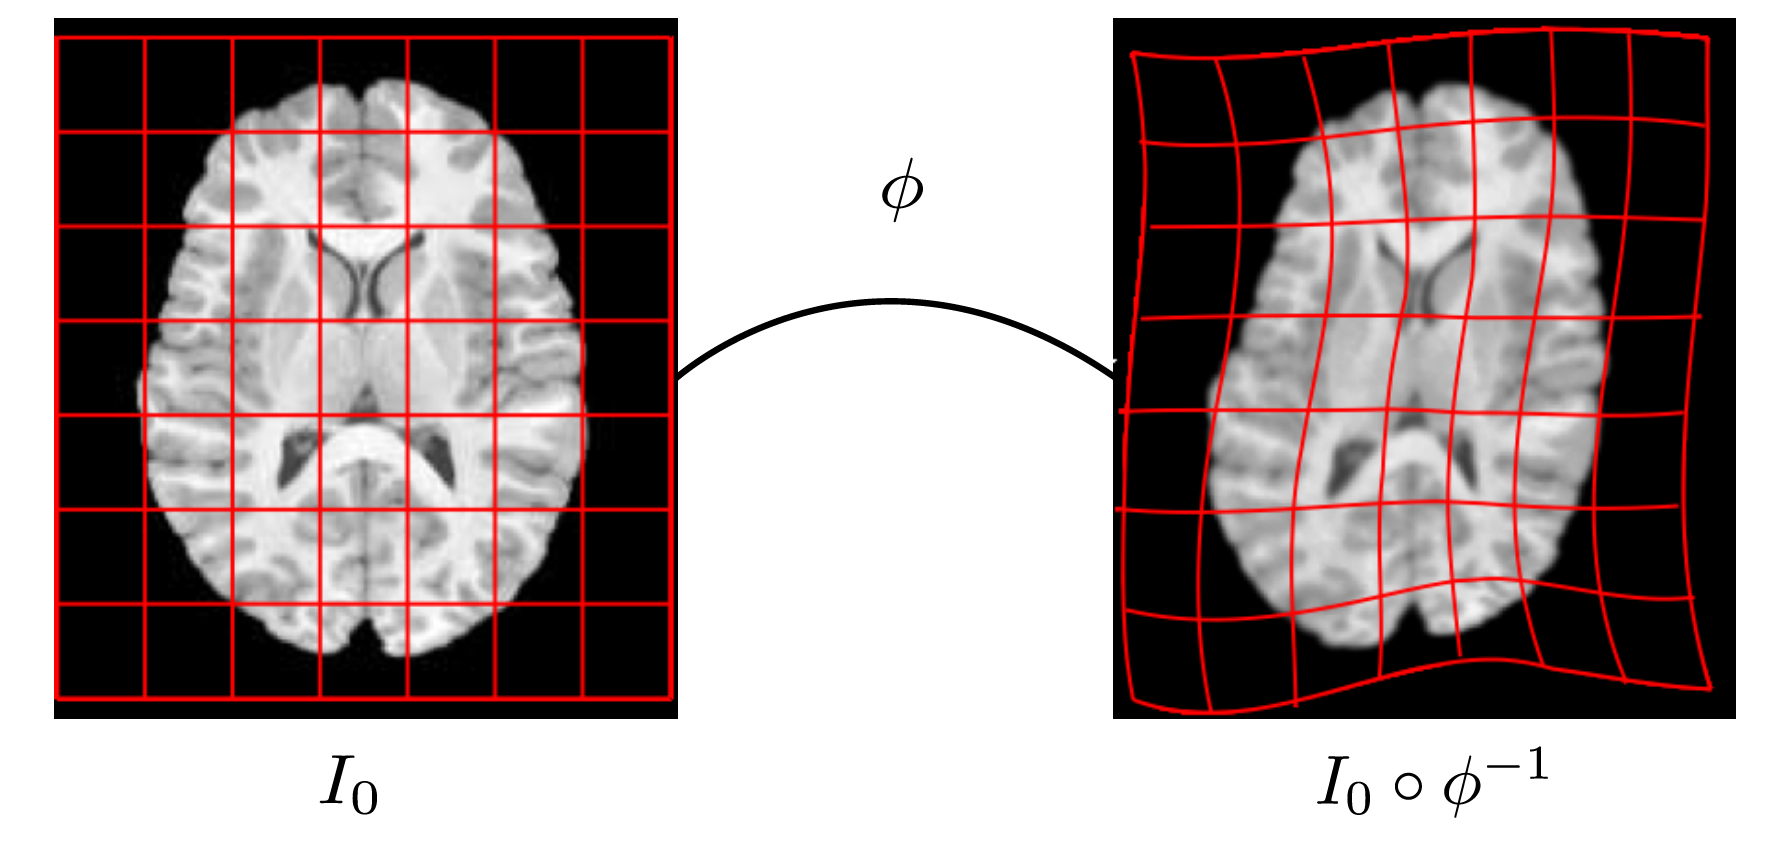
\includegraphics[scale=0.25]{figure/LDDMM.png}
\caption{Deform an axial of a 3D brain MRI image by $\phi$}
\end{figure}

\subsection{Gradient Algorithm}
To ensure that the solution lies in the space of diffeomorphisms, smoothness is achieved by defining the operator $L$ as $L=-\alpha\nabla^2+\gamma I$. In LDDMM, steepest gradient descent approach is used to perform the minimization in energy function and the velocity field at each gradient descent iteration $k$ is updated with
\begin{equation*}
    v^{k+1}(t)=v^k(t)-\varepsilon\nabla_{v^k(t)}E(t),
\end{equation*}
where $\nabla_vE(t)$ as shown below, is the gradient of the energy function
\begin{equation}
    \nabla_vE(t)=2v(t)-K*\left(\frac{1}{\sigma^2}|D\phi_{t,1}^v|\nabla J^0_t(J^0_t-J^1_t)\right)
\end{equation}
where $J^0_t=I_0\circ\phi_{t,0}, J^1_t=I_1\circ\phi_{t,1}, \phi_{s,t}=\phi_t\circ\phi^{-1}_s, K=(L^\dagger L)^{-1}$ and $*$ is the convolution.

Let the velocity $v$ be perturbed by an $\varepsilon$ amount along direction $h$. The Gateaux variation $\partial_hE(v)$ of the energy functional is related to its Frechet derivative $\nabla_vE$ by
\begin{align*}
    \partial_hE(v)&=\lim_{\varepsilon\rightarrow 0}\frac{E(v+\varepsilon h)-E(v)}{\varepsilon}\\
    &=\int^1_0\langle\nabla_vE(t),h(t)\rangledt
\end{align*}

The variation of $E_1(v)=\int^1_0\|v_t\|^2_Vdt=\int^1_0\|Lv_t\|^2_{L^2}dt$ is given by:
\begin{equation*}
    \partial_hE_1(v)=2\int^1_0\langle v_t,h_t\rangle_Vdt.
\end{equation*}

The variation of $E_2(v)=\frac{1}{\sigma^2}\|I_0\circ\phi^v_{1,0}-I_1\|^2_{L^2}$ is
\begin{align*}
    \partial_hE_2(v)&=\frac{2}{\sigma^2}\langle I_0\circ\phi^v_{1,0}-I_1,DI_0\circ\phi^v_{1,0}\cdot\partial_h\phi^v_{1,0}\rangle_{L^2}\\
    &=\frac{2}{\sigma^2}\left< I_0\circ\phi^v_{1,0}-I_1,DI_0\circ\phi^v_{0,1}\cdot\left(-D\phi^v_{1,0}\int^1_0(D\phi^v_{1,t})^{-1}h_t\circ\phi^v_{1,t}dt\right)\right>_{L^2} &&Lemma (1)\\
    &=-\frac{2}{\sigma^2}\int^1_0\langle(I_0\circ\phi^v_{1,0}-I_1,D(I_0\circ\phi^v_{1,0})\cdot(D\phi^v_{1,t})^{-1}\cdot h_t\circ\phi^v_{1,t}\rangle_{L^2}dt
\end{align*}
\begin{lemma}
The variation of mapping $\phi^v_{s,t}$ when $v\in L^2$ is perturbed along $h\in L^2$ is given by
\begin{align*}
    \partial_h\phi^v_{s,t}&=\lim_{\varepsilon\rightarrow0}\frac{\phi^{v+\varepsilon h}_{s,t}-\phi^v_{s,t}}{\varepsilon}\\
    &=D\phi^v_{s,t}\int^t_s(D\phi^v_{s,t})^{-1}h_u\circ\phi^v_{s,u}du
\end{align*}
\end{lemma}
\begin{align*}
    \partial_hE_2(v)&=-\frac{2}{\sigma^2}\int^1_0\langle|D\phi^v_{t,1}|(I_0\circ\phi^v_{t,0}-I_1\circ\phi^v_{t,1}),D(I_0\circ\phi^v_{t,0})h_t\rangle_{L^2}dt\\
    &=-\frac{2}{\sigma^2}\int^1_0\langle|D\phi^v_{t,1}|(J^0_t-j^1_t)\nabla J^0_t,h_t\rangle_{L^2}dt\\
    &=-\int^1_0\left< K\left(\frac{2}{\sigma^2}|D\phi^v_{t,1}|(J^0_t-J^1_t)\nabla J^0_t\right),h_t\right>_Vdt
\end{align*}
where the subscript $V$ indicates the gradient is in the space $V$.

Collecting terms, the gradient of the energy functional is thus
\begin{equation*}
    \nabla_vE_t=2v_t-K\left(\frac{2}{\sigma^2}|D\phi^v_{t,1}|\nabla J^0_t(J^0_t-J^1_t)\right )
\end{equation*}
The optimizing velocity field satisfies the Euler-Lagrange equation
\begin{equation*}
    \partial_hE(\hat{v})=\int^1_0\left<2\hat{v}_t-K\cdot\left(\frac{2}{\sigma^2}|D\phi^\hat{v}_{t,1}|\nabla|J^0_t(J^0_t-J^1_t)\right),t_t\right>_Vdt=0,
\end{equation*}
since $h$ is arbitrary in $L^2([0,1],V)$ we get Eq.(4).

In the numerical implementation of LDDMM, the time parameter $t$ of the flow is discretized with a fixed total number of time steps $T$, where $T=10$ is selected as the default descent to terminate with a higher final mismatch error $\|I_0\circ\phi^{-1}-I_1\|^2_{L^2}$ between the registered atlas image and the target image. 

The convolution operation in Eq.(4) is calculated in Fourier domain. The operator $K$ acts as a low pass filter at each iteration of gradient descent and the parameters $\alpha$ and $\gamma$ controls the amount of smoothing and the elasticity of the deformation. Selection of these parameters depends on the size of the deformation necessary to register the features of the atlas image to the features of the target image.

\section{Metric Matching}
\subsection{Dewitt metric and Ebin metric}
\begin{definition}
The DeWitt metric is a one-parameter family of metrics defined on $\mathrm{Met}(\Omega)$ as follows:
\begin{itemize}
    \item The split metric on $\operatorname{Met}(M)$:
    \begin{equation*}
    G^\lambda_g(u,v)=\int_\Omega\left(\mathrm{tr}(g^{-1}u_0g^{-1}v_0)+\lambda\mathrm{tr}(g^{-1}u)\mathrm{tr}(g^{-1}v)\right)\mu_g,
    \end{equation*}where $g\in\mathrm{Met}(\Omega), u,v\in T_g\mathrm{Met}(\Omega), \lambda>0, u_0=u-\frac{1}{2}\mathrm{tr}(g^{-1}u)g, v_0=v-\frac{1}{2}\mathrm{tr}(g^{-1}v)g$ are called the traceless part of $u,v$ and $\mu_g$ is the volume form on $\Omega$ induced by $g$.
    \item The split metric on $\operatorname{Sym}_+(M)$:
    \begin{equation*}
    \langle U,V\rangle_A=\mathrm{tr}(A^{-1}U_0A^{-1}V_0)\sqrt{\det A}+\lambda\mathrm{tr}(A^{-1}U)\mathrm{tr}(A^{-1}V)\sqrt{\det A},
    \end{equation*}
    where $A\in\mathrm{Sym}_+(n), U,V\in T_A\mathrm{Sym}_+(n),$ and $U_0=U-\frac{1}{n}\mathrm{tr}(A^{-1}U)A,  V_0=V-\frac{1}{n}\mathrm{tr}(A^{-1}V)A$ are called the traceless part of $U,V$ and $\sqrt{\det A}$ is the volume form induced by $A$.
\end{itemize}
\end{definition}

When $\lambda=\frac{1}{n}$, this metric gives exactly the induced Ebin metric on $\mathrm{Sym}_+(n)$, which means Ebin metric is a special case of DeWitt metric.

\begin{definition}
The Ebin metric is the Riemannian metric on $\mathrm{Sym}_+(n)$ given by
\begin{equation*}
    \left<U,V\right>_A=\mathrm{tr}(A^{-1}UA^{-1}V)\sqrt{\mathrm{det}(A)},
\end{equation*}
where $A\in\mathrm{Sym}_+(n)$ and $U,V\in T_A\mathrm{Sym}_+(n)=\mathrm{Sym}_+(n)$.
\end{definition}

\begin{proof}
\begin{align*}
    \langle U,V\rangle_A&=\mathrm{tr}(A^{-1}U_0A^{-1}V_0)\sqrt{\det A}+\frac{1}{n}\mathrm{tr}(A^{-1}U)\mathrm{tr}(A^{-1}V)\sqrt{\det A}\\
    &=\mathrm{tr}\left(A^{-1}\left(U-\frac{1}{n}\mathrm{tr}(A^{-1}U)A\right)A^{-1}\left(V-\frac{1}{n}\mathrm{tr}(A^{-1}V)A\right)\right)\sqrt{\det A}+\frac{1}{n}\mathrm{tr}(A^{-1}U)\mathrm{tr}(A^{-1}V)\sqrt{\det A}\\
    &=\mathrm{tr}\left(\left(A^{-1}U-\frac{1}{n}\mathrm{tr}(A^{-1}U)I\right)\left(A^{-1}V-\frac{1}{n}\mathrm{tr}(A^{-1}V)I\right)\right)\sqrt{\det A}+\frac{1}{n}\mathrm{tr}(A^{-1}U)\mathrm{tr}(A^{-1}V)\sqrt{\det A}\\
    &=\left[\mathrm{tr}(A^{-1}UA^{-1}V)-\frac{1}{n}\mathrm{tr}(A^{-1}U)\mathrm{tr}(A^{-1}V)-\frac{1}{n}\mathrm{tr}(A^{-1}V)\mathrm{tr}(A^{-1}U)+\frac{1}{n^2}\mathrm{tr}(A^{-1}U)\mathrm{tr}(A^{-1}V)n\right]\sqrt{\det A}\\
    &+\frac{1}{n}\mathrm{tr}(A^{-1}U)\mathrm{tr}(A^{-1}V)\sqrt{\det A}\\
    &=\left[\mathrm{tr}(A^{-1}UA^{-1}V)-\frac{1}{n}\mathrm{tr}(A^{-1}U)\mathrm{tr}(A^{-1}V)\right]\sqrt{\det A}+\frac{1}{n}\mathrm{tr}(A^{-1}U)\mathrm{tr}(A^{-1}V)\sqrt{\det A}\\
    &=\mathrm{tr}(A^{-1}UA^{-1}V)\sqrt{\det A}
\end{align*}
\end{proof}


\subsection{Inexact density matching}
For inexact metric matching, given two Riemannian metrics $g_0$ and $g_1$ in $\mathrm{Met}(\Omega)$, we are aiming to find the optimal diffeomorphism $\phi\in\mathrm{Diff}(\Omega)$ that minimizes the following energy functional w.r.t. the information metric $G^I_\phi(U,U)=\int_\Omega\langle-\Delta u,u\rangle$:
\begin{equation*}
    E(\phi)=\sigma \mathrm{dist}^2(\phi_*f_0,f_1)+\mathrm{dist}^2(\phi_*g_0,g_1)
\end{equation*}
where $\sigma>0$ is a constant, $f_0, f_1$ are called the regularization parameters, dist is the distance function for the DeWitt metric on the space of metrics $\mathrm{Met}(\Omega)$ and $\phi_*$ denotes the push-forward group action given by
\begin{equation*}
    \phi_*g_0=(\phi^{-1})^*g_0=(D\phi^{-1})^T(g_0\circ\phi^{-1})(D\phi^{-1})
\end{equation*}

The gradient of $E$ at $\phi$ transported to the identity with respect to the information metric $G^I_\phi(U,U)=\int_\Omega\langle-\Delta u,u\rangle$ is given as follows:
\begin{equation*}
    v=-\Delta^{-1}(\nabla E(\phi)\circ\phi^{-1})
\end{equation*}
where $\nabla E(\phi)\circ\phi^{-1}$ is the usual gradient of $E$ at $\phi$ transported to the identity w.r.t. the standard $L^2$ metric.

\begin{remark}
We aim to use the geodesic distance of the Ebin metric as a similarity measure for diffeomorphic Riemannian metric registration. Therefore, we fix a background metric $\bar g$ with corresponding volume density $\bar\mu$ on our parameter domain $\Omega$. Using $\bar g$, we can express any Riemannian metric $g$ on $\Omega$ as a field of matrices $A(x)$ and we can express both the Ebin metric and the geodesic distance of the Ebin metric using this representation.

Note that these terms are in fact independent of the choice of background metric, due to the invariance of the Ebin metric.

For $A,B\in\mathrm{Sym}_+(n)$, the space of symmetric, positive definite, $n$ by $n$ matrices, the Riemannian distance w.r.t. the Ebin metric is given by
\begin{equation*}
    \mathrm{dist}_E(A,B)=\sqrt{\int_{\Omega} d(A(x),B(x))^2 \bar \mu(x) }
\end{equation*}
where $d$ denotes the geodesic distance on the space of symmetric matrices defined below:
\begin{align*}
    d(A,B)^2 &=  \frac{16}{n}\left( \sqrt{\operatorname{det}(A)}  -2\sqrt[4]{\operatorname{det}(A)}\sqrt[4]{\operatorname{det}(B)}  \cos{\theta} 
+\sqrt{\operatorname{det}(B)}\right), \\
\text{where }\theta &=  \min\left\{\pi, \frac{\sqrt{n\operatorname{tr}(K_0^2)}}{4}\right\}, K=\operatorname{log}(A^{-1}B)\text{ and } K_0=K-\tfrac{1}{n} \, \operatorname{tr}(K)I\,.
\end{align*}
\end{remark}

\begin{remark}
Below is the reason why $K_0=K-\frac{1}{n}\operatorname{tr}(K)I$ is call traceless part of $K$:
\begin{align*}
    K_0&=K-\frac{1}{n}\operatorname{tr}(K)I\\
   \operatorname{tr}(K_0)&=\operatorname{tr}(K-\frac{1}{n}\operatorname{tr}(K)I)\\
   \operatorname{tr}(K_0)&=\operatorname{tr}(K)-\operatorname{tr}(\frac{1}{n}\operatorname{tr}(K)I)\\
   \operatorname{tr}(K_0)&=\operatorname{tr}(K)-\frac{1}{n}\operatorname{tr}(K)\operatorname{tr}(I)&&\triangleright I \text{ is a }n\times n \text{ identity matrix}\\
   \operatorname{tr}(K_0)&=\operatorname{tr}(K)-\frac{1}{n}\operatorname{tr}(K)n\\
   \operatorname{tr}(K_0)&=\operatorname{tr}(K)-\operatorname{tr}(K)\\
   \operatorname{tr}(K_0)&=0
\end{align*}
\end{remark}

\begin{remark}
Given $K_0=K-\frac{1}{n}\operatorname{tr}(K)I,K=\log{(A^{-1}B)}$, $\mathrm{tr}(K^2_0)$ is given by
\begin{align*}
    K_0^2&=K^2-\frac{2}{n}\mathrm{tr}(K)K+\frac{1}{n^2}\mathrm{tr}^2(K)I\\
    \mathrm{tr}(K^2_0)&=\mathrm{tr}(K^2)-\frac{2}{n}\mathrm{tr}(K)\mathrm{tr}(K)+\frac{1}{n^2}\mathrm{tr}^2(K)\mathrm{tr}(I)\\
    \mathrm{tr}(K^2_0)&=\mathrm{tr}(K^2)-\frac{2}{n}\mathrm{tr}(K)^2+\frac{1}{n^2}\mathrm{tr}^2(K)n\\
    \mathrm{tr}(K^2_0)&=\mathrm{tr}(K^2)-\frac{1}{n}\mathrm{tr}^2(K)\\
    \mathrm{tr}(K^2_0)&=\mathrm{tr}(K^2)-\frac{1}{n}\log^2(\det(A^{-1}B))&&\triangleright \mathrm{tr}(\log(K))=\log(\det(K))\cite{jacobi}
\end{align*}
\end{remark}

\begin{remark}
The energy function is given by 
\begin{equation*}
    E(\phi)=\mathrm{dist}^2_E(\phi^*A,B)
\end{equation*}

By introducing some additional notation, we can write $d(A,B)^2$ as
\begin{equation*}
    d(A,B)^2=\frac{16}{n}(\alpha^2-2\alpha\beta\cos(\theta)+\beta^2),
\end{equation*}
where $\alpha=\sqrt[4]{\operatorname{det}(A)},\beta=\sqrt[4]{\operatorname{det}(B)},\theta=\min\left\{\pi, \frac{\sqrt{n\operatorname{tr}(K_0^2)}}{4}\right\}$.

In order to perform this minimization numerically, we need to calculate the gradient of this functional at $\phi=\mathrm{id}$, which is given by
\begin{equation*}
    \delta\left(d(A,B)^2\right)(\delta A)=\frac{16}{n}(2\alpha\delta(\alpha(A))(\delta A)-2\delta(\alpha(A))(\delta A)\beta\cos(\theta)+2\alpha\beta\sin(\theta)\delta(\theta(A))(\delta A)),
\end{equation*}
where $\delta$ is the differential operator. The $\delta\left(d(A,B)^2\right)(\delta A)$ above can give us the directional derivative in the direction of $\delta A$.

Replacing $A$ with $\phi^*A$, we can have
\begin{equation}
    \delta\left(d(\phi^*A,B)^2\right)(\delta\phi^* A)=\frac{16}{n}(2\alpha\delta(\alpha(\phi^*A))(\delta \phi^*A)-2\delta(\alpha(\phi^*A))(\delta \phi^*A)\beta\cos(\theta)+2\alpha\beta\sin(\theta)\delta(\theta(\phi^*A))(\delta\phi^*A)).\label{ebinenergy}
\end{equation}

As for $\delta(\alpha(A))(\delta A)$, it's given by
\begin{align*}
    \delta(\alpha(A))(\delta A)&=\delta(\operatorname{det}(A)^\frac{1}{4})(\delta A)\\
    &=\frac{1}{4}\operatorname{det}(A)^{-\frac{3}{4}}\cdot\delta(\operatorname{det}(A))(\delta A)\\
    &=\frac{1}{4}\operatorname{det}(A)^{-\frac{3}{4}}\cdot\operatorname{tr}(\operatorname{adj}(A))(\delta A)&&\triangleright\text{Jacobi's formula}\\
    &=\frac{1}{4}\operatorname{det}(A)^{-\frac{3}{4}}\cdot\operatorname{det}(A)\cdot\operatorname{tr}(A^{-1})(\delta A)\\
    &=\frac{1}{4}\operatorname{det}(A)^{\frac{1}{4}}\cdot\operatorname{tr}(A^{-1})(\delta A)
\end{align*}

Replacing $A$ with $\phi^*A$, we can have
\begin{equation}
    \delta(\alpha(\phi^*A))(\delta \phi^*A)=\frac{1}{4}\operatorname{det}(\phi^*A)^{\frac{1}{4}}\cdot\operatorname{tr}((\phi^*A)^{-1})(\delta \phi^*A).\label{alphaphia}
\end{equation}

As for $\delta \phi^*A$, it's given by
\begin{equation}
    \delta(\phi^*A)(\delta\phi)\bigg\rvert_{\phi=\operatorname{id}}=\mathcal{L}_XA=\begin{pmatrix}\mathcal{L}_XA_{11}&\mathcal{L}_XA_{12}\\\mathcal{L}_XA_{21}&\mathcal{L}_XA_{22}\end{pmatrix}.\label{lxa}
\end{equation}

More specifically,
\begin{equation*}
    \mathcal{L}_XA_{ij}=X^k\partial_k(A_{ij})+\partial_i(X^j)A_{kj}+\partial_j(X^i)A_{ik}
\end{equation*}
where $X=\delta\phi$ is induced by $\phi$.

For the 2D case, we can have the these expressions:
\begin{align*}
    \mathcal{L}_XA_{11}&=X^1\partial_1(A_{11})+X^2\partial_2(A_{11})+\partial_1(X^1)A_{11}+\partial_1(X^1)A_{21}+\partial_1(X^1)A_{11}+\partial_1(X^1)A_{12}\\
    \mathcal{L}_XA_{12}&=X^1\partial_1(A_{12})+X^2\partial_2(A_{12})+\partial_1(X^2)A_{12}+\partial_1(X^2)A_{22}+\partial_2(X^1)A_{11}+\partial_2(X^1)A_{12}\\
    \mathcal{L}_XA_{21}&=X^1\partial_1(A_{21})+X^2\partial_2(A_{21})+\partial_2(X^1)A_{11}+\partial_2(X^1)A_{21}+\partial_1(X^2)A_{21}+\partial_1(X^2)A_{22}\\
    \mathcal{L}_XA_{22}&=X^1\partial_1(A_{22})+X^2\partial_2(A_{22})+\partial_2(X^2)A_{12}+\partial_2(X^2)A_{22}+\partial_2(X^2)A_{21}+\partial_2(X^2)A_{22}
\end{align*}

By substituting Eq.(\ref{alphaphia},\ref{lxa}) into Eq.(\ref{ebinenergy}), we can have the final expression of $\delta\left(d(\phi^*A,B)^2\right)\delta(\phi^* A)$.

\begin{align*}
    \delta(\theta(A))(\delta A)&=\frac{d\left(\frac{\sqrt{n\operatorname{tr}(K^2_0)}}{4}\right)}{d(n\operatorname{tr}(K^2_0))}\cdot\frac{d(n\operatorname{tr}(K^2_0))}{d(\operatorname{tr}(K^2_0))}\cdot\delta(\operatorname{tr}(K^2_0))(\delta A)\\
    &=\frac{1}{4}\cdot\frac{1}{2}(n\operatorname{tr}(K^2_0))^{-\frac{1}{2}}\cdot n\cdot\delta(\operatorname{tr}(K^2_0))(\delta A)\\
    &=\frac{\sqrt{n}}{8}\operatorname{tr}^{-\frac{1}{2}}(K^2_0)\cdot\delta(\operatorname{tr}(K^2_0))(\delta A)
\end{align*}
\begin{align*}
    \delta(\operatorname{tr}(K^2_0))(\delta A)&=\delta\left(\operatorname{tr}(K^2)-\frac{1}{n}\log^2(\operatorname{det}(A^{-1}B))\right)(\delta A)\\
    &=\delta\left(\operatorname{tr}(\log^2(A^{-1}B))-\frac{1}{n}\log^2(\operatorname{det}(A^{-1}B))\right)(\delta A)\\
    &=\delta(\operatorname{tr}(\log^2(A^{-1}B)))(\delta A)-\frac{1}{n}\delta\left(\log^2(\operatorname{det}(A^{-1}B))\right)(\delta A)\\
\end{align*}
\begin{align*}
    \delta(\operatorname{tr}(\log^2(A^{-1}B)))(\delta A)&=\frac{d\operatorname{tr}(\log^2(A^{-1}B))}{d\log^2(A^{-1}B)}\cdot\frac{d\log^2(A^{-1}B)}{d\log(A^{-1}B)}\cdot\frac{d\log(A^{-1}B)}{d(A^{-1}B)}\cdot\frac{d(A^{-1}B)}{dA^{-1}}\cdot\delta(A^{-1})(\delta A)\\
    &=I\cdot2\log(A^{-1}B)\cdot\cdot B\cdot(-A^{-1}A^{-1})(\delta A)
\end{align*}
\begin{align*}
    \delta\left(\log^2(\operatorname{det}(A^{-1}B))\right)(\delta A)&=\frac{d(\log^2(\det(A^{-1}B))}{d(\log(\det(A^{-1}B))}\cdot\frac{d(\log(\det(A^{-1}B))}{d\det(A^{-1}B)}\cdot\frac{d\det(A^{-1}B)}{dA^{-1}B}\cdot\frac{dA^{-1}B}{dA^{-1}}\cdot\delta(A^{-1})(\delta A)\\
    &=2\log(\det(A^{-1}B))\cdot\frac{1}{\det(A^{-1}B)}\cdot\det(A^{-1}B)((A^{-1}B)^{-1})^T\cdot B\cdot(-A^{-1}A^{-1})(\delta A)\\
    &=2\log(\det(A^{-1}B))\cdot((A^{-1}B)^{-1})^T\cdot B\cdot(-A^{-1}A^{-1})(\delta A)\\
    &=2\log(\det(A^{-1}B))\cdot(B^{-1}A)^T\cdot B\cdot(-A^{-1}A^{-1})(\delta A)\\
    &=2\log(\det(A^{-1}B))\cdot A^T(B^{-1})^T\cdot B\cdot(-A^{-1}A^{-1})(\delta A)\\
    &=2\log(\det(A^{-1}B))\cdot A^T(B^T)^{-1}\cdot B\cdot(-A^{-1}A^{-1})(\delta A)\\
    &=2\log(\det(A^{-1}B))\cdot AB^{-1}\cdot B\cdot(-A^{-1}A^{-1})(\delta A)\\
    &=-2\log(\det(A^{-1}B))\cdot A^{-1}(\delta A)\\
\end{align*}
\begin{align*}
    \log(A)&=\sum^\infty_{k=1}(-1)^{k+1}\frac{(A-I)^k}{k}\\
    &=(A-I)-\frac{(A-I)^2}{2}+\frac{(A-I)^3}{3}-\cdots\\
    \frac{d\log(A)}{dA}&=\frac{d(A-I)}{dA}-\frac{1}{2}\cdot\frac{d(A-I)^2}{d(A-I)}\cdot\frac{d(A-I)}{dA}+\frac{1}{3}\cdot\frac{d(A-I)^3}{d(A-I)}\cdot\frac{d(A-I)}{dA}-\cdots\\
    &=I-\frac{1}{2}\cdot2(A-I)\cdot I+\frac{1}{3}\cdot3(A-I)\cdot I-\cdots\\
    &=\sum^\infty_{k=0}(-1)^k(A-I)^k
\end{align*}
\end{remark}

\section{Appendix}
\subsection{Geodesic Shooting}
Given an initial velocity $v_0\in V$, the geodesic path $t\rightarrow\phi_t\in\mathrm{Diff}^\infty(\Omega)$ under the right-invariant Riemannian metric is uniquely determined by the Euler-Poincare equations(EPDiff)
\begin{equation}
    \frac{\partial v}{\partial t}=-\mathrm{ad}^\dagger_v v=-K\mathrm{ad}^*_vm=-K[(Dv)^Tm+Dmv+m\mathrm{ div } v],
\end{equation}
where $D$ denotes the Jacobian matrix, and the operator $\mathrm{ad}^*$ is the dual of the negative Lie bracket of vector fields,
\begin{equation*}
    \mathrm{ad}_vw=-[v,w]=Dvw-Dwv.
\end{equation*}

By integrating equation (4) forward in time, we generate a time-varying velocity $v_t:[0,1]\rightarrow V$, which itself is subsequently integrated in time by rule $d\phi(x,t)dt=v_t\circ\phi_t(x)$ to arrive at the geodesic path, $\phi(x,t)\in\mathrm{Diff}^s(\Omega)$.

\begin{thebibliography}{99} 
\bibitem{joshi}Joshi, S.C. and Miller, M.I., 2000. \textit{Landmark matching via large deformation diffeomorphisms}. IEEE transactions on image processing, 9(8), pp.1357-1370.
\bibitem{miller}Miller, M.I., Trouvé, A. and Younes, L., 2002. \textit{On the metrics and Euler-Lagrange equations of computational anatomy}. Annual review of biomedical engineering, 4(1), pp.375-405.
\bibitem{johnson}Johnson, H.J. and Christensen, G.E., 2001, June. \textit{Landmark and intensity-based, consistent thin-plate spline image registration}. In Biennial International Conference on Information Processing in Medical Imaging (pp. 329-343). Springer, Berlin, Heidelberg.
\bibitem{tang}Ceritoglu, C., Tang, X., Chow, M., Hadjiabadi, D., Shah, D., Brown, T., Burhanullah, M.H., Trinh, H., Hsu, J., Ament, K.A. and Crocetti, D., 2013. \textit{Computational analysis of LDDMM for brain mapping. Frontiers in neuroscience}, 7, p.151.
\bibitem{beg}Beg, M.F., Miller, M.I., Trouvé, A. and Younes, L., 2005. \textit{Computing large deformation metric mappings via geodesic flows of diffeomorphisms}. International journal of computer vision, 61(2), pp.139-157.
\bibitem{pga1}Fletcher, P.T., Lu, C. and Joshi, S., 2003, June. \textit{Statistics of shape via principal geodesic analysis on Lie groups}. In 2003 IEEE Computer Society Conference on Computer Vision and Pattern Recognition, 2003. Proceedings. (Vol. 1, pp. I-I). IEEE.
\bibitem{pga2}Fletcher, P.T., Lu, C., Pizer, S.M. and Joshi, S., 2004. \textit{Principal geodesic analysis for the study of nonlinear statistics of shape}. IEEE transactions on medical imaging, 23(8), pp.995-1005.
\bibitem{hao}Hao, X., Zygmunt, K., Whitaker, R.T. and Fletcher, P.T., 2014. \textit{Improved segmentation of white matter tracts with adaptive Riemannian metrics}. Medical image analysis, 18(1), pp.161-175.
\bibitem{jacobi}Logarithm of a matrix: A Lie group theory perspective. Wikipedia. \url{https://en.wikipedia.org/wiki/Logarithm_of_a_matrix}
\bibitem{hinkle}Hinkle, J. and Joshi, S., 2013, June. \textit{Idiff: irrotational diffeomorphisms for computational anatomy}. In International Conference on Information Processing in Medical Imaging (pp. 754-765). Springer, Berlin, Heidelberg.
\bibitem{khesin}Khesin, B., Lenells, J., Misiolek, G. and Preston, S.C., 2011. \textit{Geometry of diffeomorphism groups, complete integrability and optimal transport}. arXiv preprint arXiv:1105.0643.
\bibitem{macedo}Macêdo, I. and Castro, R., 2010. Learning divergence-free and curl-free vector fields with matrix-valued kernels. IMPA.
\end{thebibliography}
\end{document}
